% Sample LaTeX file for creating a paper in the Morgan Kaufmannn two
% column, 8 1/2 by 11 inch proceedings format.
\documentstyle[proceed]{article}

\usepackage{microtype}
\usepackage{graphicx}
\usepackage{subfigure}
\usepackage{booktabs} % for professional tables
\usepackage{bm}
\usepackage{amsmath}
\usepackage{amsfonts}
\usepackage{amstext}
\usepackage[usenames,dvipsnames]{color}
\usepackage{colortbl}
\definecolor{mygray}{gray}{.9}
\usepackage{hyperref}
\newcommand{\theHalgorithm}{\arabic{algorithm}}


\title{A Bayesian Hierarchical Model for Personalized Apparel Recommendation}

\author{} % LEAVE BLANK FOR ORIGINAL SUBMISSION.
          % UAI  reviewing is double-blind.

% The author names and affiliations should appear only in the accepted paper.
%
%\author{ {\bf Harry Q.~Bovik\thanks{Footnote for author to give an
%alternate address.}} \\
%Computer Science Dept. \\
%Cranberry University\\
%Pittsburgh, PA 15213 \\
%\And
%{\bf Coauthor}  \\
%Affiliation          \\
%Address \\
%\And
%{\bf Coauthor}   \\
%Affiliation \\
%Address    \\
%(if needed)\\
%}




\begin{document}

\maketitle

\begin{abstract}
Abstract.
\end{abstract}

\section{Introduction(Jerry)}
\label{sec:intro}
Real-world organizations in business domains operate in a multi-item, multi-level environment. Items and their corresponding information collected by these organizations often reflect a hierarchical structure. For examples, products in retail stores are usually stored in hierarchical inventories. News on web pages is created and placed hierarchically in most websites. These hierarchical structures and the data within them provide a large amount of information when building effective recommendation systems. Especially in e-commerce domain, all products are displayed in a site-wide hierarchical catalog and how to build an accurate recommendation engine on top of it becomes one of the keys to majority companies' business success nowadays. 

However, how to utilize the rich information behind hierarchical structures to make personalized and accurate product recommendations still remains challenging due to the unique characteristics of hierarchical structures and the modeling trade-offs arising from them. Briefly, most well-established recommendation algorithms cannot naturally take hierarchical structures as additional inputs and flatting hierarchical structures usually doesn't work well. It will not only blow up the entire feature space but introduce noise when training the recommendation models. On the other hand, completely ignoring the hierarchies will lead to recommendation inaccuracies. The most common way to alleviate this problem is to feed every piece of data from the hierarchy into a complex deep neural network and hope the network itself can figure out a way to use the hierarchical knowledge. However, such approaches usually behave more like black boxes. They are difficult to debug and cannot provide any interpretation of their intermediate results and outcomes.

In this work, we propose and develop a hierarchical Bayesian, a.k.a., \emph{HBayes}, modeling framework that is able to flexibly capture various relations between items in hierarchical structures from different recommendation scenarios. By introducing latent variables, all hierarchical structures are encoded as conditional independence in HBayes graphical models. Moreover, we develop a variational inference algorithm for learning parameters of HBayes. 

To illustrate the modeling power of the proposed HBayes approach, we introduce HBayes by using a real-world apparel recommendation problem as an example. As an illustration, we consider apparel styles, product brands and apparel items,  and form them into a three-level hierarchical structure. We add additional latent variables as the apparel style membership variables to capture the diverse and hidden style properties of each brand. Furthermore, we include user-specific features into HBayes and extend HBayes into the supervised learning setting where users feedback actions such as clicks and conversions are incorporated. Please note that our HBayes framework is not only limited to apparel recommendation and at the end, we show its flexibility and effectiveness on a music recommendation problem as well.

Overall this paper makes the following contributions:

\begin{itemize}
\item It presents a generalized hierarchical Bayesian learning framework to learn models from rich data with hierarchies.
\item It provides a variational inference algorithm that can learn the model parameters with few iterations.
\item We evaluate our HBayes and its benefits comprehensively in tasks of apparel recommendation on a real-world data set. 
\item We test our framework in different recommendation scenarios to show its generalization and applicability.
\end{itemize}

The remainder of the paper is organized as follows: Section \ref{sec:related} provides a review of existing recommendation algorithms and their extensions in hierarchal learning settings. Section \ref{sec:method} introduces the notations and our generalized HBayes learning framework and its variational inference algorithm. In Section \ref{sec:experiment}, we conduct experiments in a real-world e-commerce data set to show the effectiveness of our proposed recommendation algorithm in different aspects. In addition, we test our model on a music recommendation data set to illustrate the generalization and extended ability of HBayes. We summarize our work and outline potential future extensions in Section \ref{sec:conclusion}.




\section{Related Work(Chris)}
\label{sec:related}
\subsection{Recommender Systems}

With the explosive growth of digital information over the Internet, the recommender system is considered to be one of the most effective approaches to overcome such information overload. Traditional recommendation algorithms such as item-based approaches learn interactions between users and items and recommend items to users who share similar historical behaviors: collaborative filtering \cite{Sarwar:2001:ICF:371920.372071,Su:2009:SCF:1592474.1722966} and matrix factorization \cite{Rendle:2010:FPM} are both effective approaches under this category.  Content-based approaches including \cite{2011rsh..book...73L,Liu:2011,Yuan:2015} take use of the auxiliary information of both users and items in the content spaces to recommend similar items.  Furthermore, session based recommender system is developed by analyzing user session information and user visiting patterns \cite{Gultekin_acollaborative,Tang_review:2013}. Session based recommendation techniques take time as an additional dimension, which aims at explicitly modeling user interests over time slices. \cite{Koren:2010} develops a collaborative filtering type of approach with predictions from static average value combining with a dynamic changing factor. \cite{Yin:2011} proposes a user-tag-specific temporal interest model to track user interests over time by maximizing the time weighted data likelihood.  For better personalization, \cite{Guy:2009} proposes an item-based recommender system to utilize each user's social network information. 

\subsection{Bayesian Approaches for Recommendation}

Recently, there are works using Bayesian inferencing for recommender systems. \cite{rendle2009bpr} combines the Bayesian inference and matrix factorization together for learning users implicit feedbacks (click \& purchase) that is able to directly optimize ranking results. \cite{Ben-Elazar:2017} and \cite{zhang2007efficient} take user preference consistency into account and develop a variational Bayesian personalized ranking model for better music recommendation.  However, none of these approaches leverage the item structural information when learning the Bayesian models.  Given the fact that hierarchical structures widely exist in real-world recommendation scenarios such as e-commerce, social network, music, etc. failing to utilize such structural information typically makes the Bayesian approaches inefficient and ineffective.  

\subsection{Hierarchical Recommender Systems}

Hierarchical information for recommender systems, as mentioned, is a natural yet powerful entity structure that encodes human knowledge by means of tree based dependency constraints between items and the corresponding hyper-parameters for recommender systems.  Recommender system hierarchies could be explicit or implicit, and there are a few approaches take use of such information in order to recommend items to users who have explicitly visited other hierarchically related items or shown preferences to items that are hierarchically belonging to the same sub-categories.  In social tagging systems, Shepitsen et.al. \cite{shepitsen2008personalized} relies on the hierarchies generated by user-taggings, a.k.a folksonomies to build a better personalized recommender system.  In e-commerce, Wang et.al. \cite{wang2018exploring} introduces a hierarchical matrix factorization approach that exploits the intrinsic hierarchical information to alleviate cold start and data sparsity problems.  Despite the fact that these hierarchical recommender systems have received some success, there are still some challenges such like: 1. how to design the hierarchical structure and learn such structure efficiently if it is not completely explicit; 2. how to better understand the implicit hierarchical topologies discovered by recommendation approaches and ... all remain unsolved issues.

In this work, we focus on building a generic recommender system that combines the hierarchical structural information as well as the Bayesian inference to better tackle the recommendation problem.  Bayesian learning scheme takes account of both the user preferences and product hidden structural properties. It is able to recommend products that align to users' long term tastes. Meanwhile, the learned latent variables can be well interpreted and explained, which grants us the capability to analyze and understand users interests and preference.

\section{Methodology(Jerry)}
\label{sec:method}

\section{Experiment(Chris)}
\label{sec:experiment}
In this section, we conduct several experiments on two data sets: (1) our case study: the real-world e-commerce apparel data set; (2) the publicly available music data set.  For both data sets, we compare HBayes against several other \emph{state-of-the-art} recommendation approaches which are briefly mentioned as follows:

{\noindent\textbf{HSR} \cite{wang2015exploring} is an item-based recommendation approach that employs a special non-negative matrix factorization for exploring the implicit hierarchical structure of users and items so the user preference towards certain products is better understood.  \newline %We adopt HSR  as one baseline.
\textbf{HPF} \cite{gopalan2015scalable} generates a hierarchical \emph{Poisson} factorization model for better modeling users' rating towards certain items based upon each one's latent preferences.  Unlike proposed HBayes, HPF does not leverage the entity content feature for constructing the hierarchical structure.  \newline %We adopt HPF as another baseline. \newline
\textbf{SVD++} \cite{mnih2008probabilistic, koren2008factorization} combines the collaborative filtering and latent factor approaches, so to provide the more accurate neighboring based recommendation results.  \newline % We adopt SVD++ as another baseline. \newline
\textbf{CoClustering} \cite{george2005scalable} is a collaborative filtering approach based on weighted co-clustering improvements that simultaneously cluster users and items.  \newline %We adopt CoClustering as another baseline. \newline
\textbf{Factorization Machine (FM)} \cite{rendle2010factorization,rendle2012factorization} combines support vector machines (SVM) with factorization models.  It takes the advantage of SVM meanwhile overcomes the feature sparsity issues.  In this paper, we adopt the LibFM implementation mentioned in \cite{rendle2012factorization} specifically as another baseline. \newline
\textbf{LambdaMART} \cite{burges2010ranknet} is the boosted tree version of LambdaRank \cite{donmez2009local}, which is based on RankNet \cite{burges2005learning}.  LambdaMART proves to be a very successful approach for ranking as well as recommendation.  %We include LambdaMART as another baseline. \newline}

\subsection{Evaluation Metrics}
Throughout the experiments, we compare HBayes against other baselines on the testing held-out dataset under the 5-folds cross-validation settings.  For each fold, after fitting the model on the training set, we rank on the test set by each model, and generate the top M samples with maximal ranking scores for recommendation.  Regarding metrics, we adopt precisions, recalls as well as F1-scores for evaluating the item retrieval quality and normalized discounted information gain (NDCG) for evaluating the recommendation ranking quality.  More specifically, each metric mentioned is defined as:

\begin{eqnarray}
\text{Precision@K} & = & \frac{\text{\# of products clicked in top K}}{\text{K}} \nonumber \\
\text{Recall@K}      & = & \frac{\text{\# of products clicked in top K}}{\text{\# of products the user clicked}} \nonumber \\
\text{F1-score@K} & = & 2\cdot\frac{\text{Precision@K} \cdot \text{Recall@K}}{\text{Precision@K} + \text{Recall@K}}  \nonumber
\end{eqnarray}

discounted cumulative gain (DCG) measures the ranking quality based on the item positions from the resulting list, which is defined as:
\begin{eqnarray}
\text{DCG@K} & = & \sum_{i=1}^K\frac{r_i}{\log_2(i+1)} =  r_1 + \sum_{i=2}^K\frac{r_i}{\log_2(i+1)}\nonumber
\end{eqnarray}

re-rank all potential products to produce the ideal maximal possible DCG through out first K items, and its corresponding DCG score is called the ideal discounted cumulative gain (IDCG).  By using both DCG and IDCG, the normalized discounted cumulative gain (NDCG) is defined as:

\begin{eqnarray}
\text{NDCG@K} & = & \frac{\text{DCG@K}}{\text{IDCG@K}}\nonumber
\end{eqnarray}

\subsection{Recommendation on Apparel Data}
The first apparel data set is collected from a large e-commerce company.  In this dataset, each sample represents a particular apparel product which is recorded by various features including: categories, titles, and other properties, etc.  Meanwhile, the user click information is also recorded and translated into data labels. Throughout the experiment, positive labels indicate that certain recommended products are clicked by the user, whereas negative samples indicate that the recommended products are skipped by the user which usually implies that the user is `lack of interest' towards that certain item.  By data cleaning and preprocessing: (1) merging duplicated histories; (2) removing users of too few records, the post-processed data set ends up with $\mathbf{895}$ users, $\mathbf{81223}$ products, $\mathbf{5535}$ brands with $\mathbf{380595}$ uniquely observed user-item pairs.  In average, each user has $\mathbf{425}$ products records, ranging from $\mathbf{105}$ to $\mathbf{2048}$, and $\mathbf{61.2\%}$ of the users have fewer than $\mathbf{425}$ product clicking records.  For each item, we encode the popularity and category features into a $\mathbf{20}$ dimensional feature vector; title and product property into a $\mathbf{50}$ dimensional feature vector.  Combining with all features, the total dimension of each sample ends up with $\mathbf{140}$.

\subsubsection{Feature Analysis}
The apparel data are composed of four types of features: (1) product popularity; (2) product category; (3) product title; (4) product properties.  We briefly explain each feature's physical meaning and how we process the data as follows:

\textbf{Product Popularity} (POP): product popularity is a measure of the prevalence of certain items in the dataset. In general, customers have preferences for a particular product during a period of time. This phenomenon is pretty common for apparel products (\emph{e.g.} apparels' popularity in certain styles may be affected by the public, especially by those important public figures). For a particular product $i$, the popularity is defined as: $\mathrm{\scriptsize POP}_{i} \coloneqq \frac{n_{x_i}}{\mathcal{N}_\mathbf{x}}$, where $n_{x_i}$ are the number of orders or the contribution of gross merchandise volume (GMV) for product $i$,  and $\mathcal{N}_\mathbf{x} = \sum_{\forall x_i}n_{x_i}$ is the summation of $n_{x_i}$ across all products in the dataset. \newline

\textbf{Product Category} (CID): In e-commerce, items are clustered into different groups based on the alliance/ similarity of the item functionalities and utilities.  In e-commerce websites, such an explicit hierarchy usually exists.  We encode each item's category into a high dimensional vector via one-hot encoding and adjust the feature weights by the popularity of such category. \newline

\textbf{Product Title} (TITLE): product titles are created by vendors and they are typically in the forms of natural languages indicating the item functionality and utility.  Examples could be like `\emph{INMAN short sleeve round neck triple color block stripe T-shirt 2017}'.  We preprocess the product titles by generating the sentence embedding based on \cite{de2016representation}.  The main idea is to average the wording weights in the title sentence based on the inverse document frequency (IDF) value of each individual word involved. \newline

\textbf{Product Property Features} (PROP): other product metadata features are also provided in the apparel dataset. For instance, the color feature of items takes values such like: `black', `white', `red', etc, and the sizing feature takes values such like: `S', `M', `L', `XL', etc.  Similar to category features, product properties are first encoded into binary vectors $\bm{x}_i \in \{0, 1\}^{|N|}$, where $N$ denotes the set of all possible product values.  Then the property binary vectors are hashed into fixed length ($50$) vectors. \newline

On one hand, by utilizing more features HBayes in general reaches better performance in terms of precision-recall metrics.  We report PR-AUC in the table (\ref{tab:features_cmp}) to prove this argument; on the other hand, more features need more training time.  Figure (\ref{fig:train_time_cmp}) reports the changes in likelihood against training time cost (in minutes) for each feature using cases\footnote{The experiment is conducted via the same Linux Qual core 2.8 GHz Intel Core i7 MacBook with 16 Gigabytes of memory}. It is shown that by only taking POP features, model spends less than 5 minutes to converge while taking POP+CID+TITLE+PROP features, the model needs more than 4 hours in training.   

\begin{table}[htb]
\centering
\scalebox{0.85}{
\begin{tabular}{l|c}
\toprule
\textbf{Features} & \textbf{PR AUC} \\
\hline
POP & 0.0406 \\
\rowcolor{mygray}
POP+CID & 0.0414 \\
POP+CID+TITLE & 0.0489 \\
\rowcolor{mygray}
POP+CID+TITLE+PROP & 0.0491 \\
\bottomrule
\end{tabular}}
\caption{Model performance under different feature combinations in terms of PR AUC}
\label{tab:features_cmp}
\end{table}

\begin{figure*}[!htb]
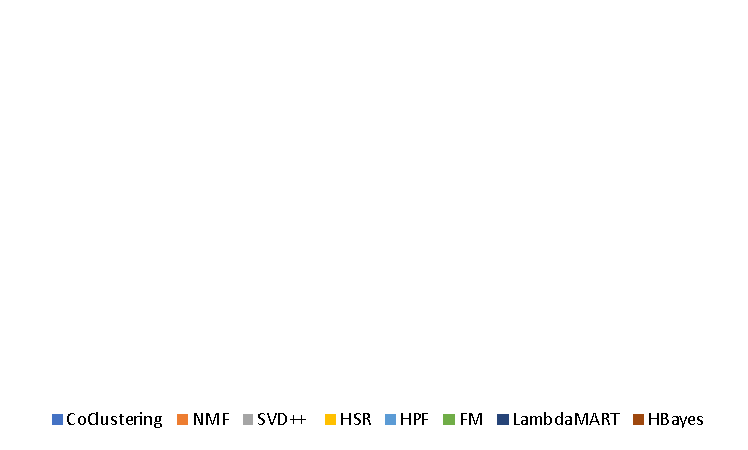
\includegraphics[width=0.7\linewidth]{fig/legend}
\end{figure*}

\begin{figure*}[!htb]
\minipage{0.32\textwidth}
  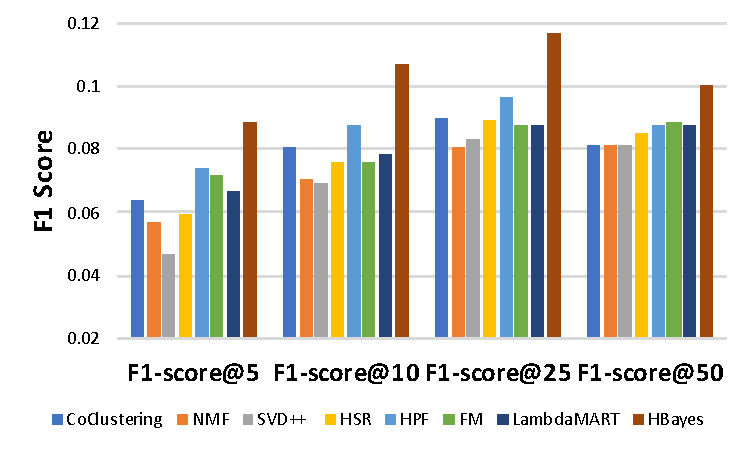
\includegraphics[width=\linewidth]{fig/F1-score_jd}
  \caption{F1@K on \emph{Apparel} data.}
  \label{fig:perf_cmp_F1_apparel}
\endminipage\hfill
\minipage{0.32\textwidth}
  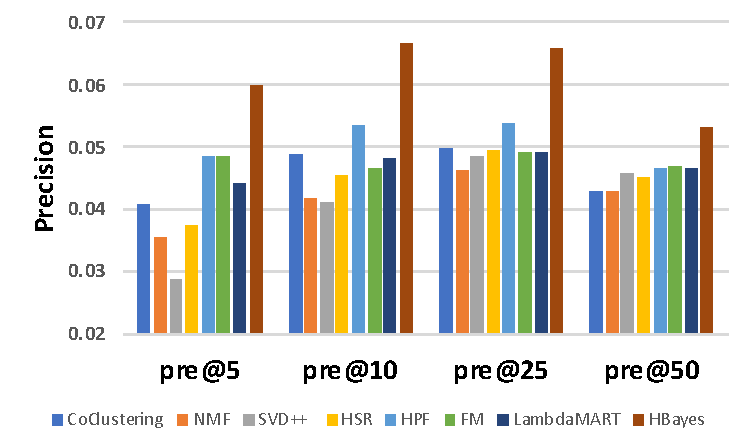
\includegraphics[width=\linewidth]{fig/precision_jd}
  \caption{Precision@K on \emph{Apparel} data.}
  \label{fig:perf_cmp_precision_apparel}
\endminipage\hfill
\minipage{0.32\textwidth}%
  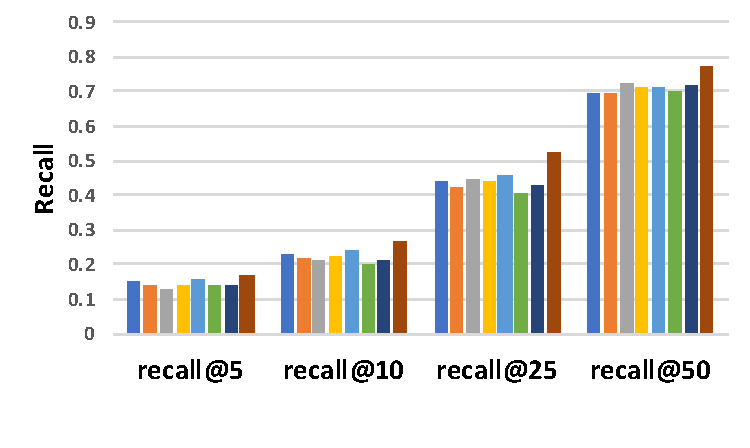
\includegraphics[width=\linewidth]{fig/recall_jd}
  \caption{Recall@K on \emph{Apparel} data.}
  \label{fig:perf_cmp_recall_apparel}
\endminipage
\end{figure*}


\begin{figure*}[!htb]
\minipage{0.32\textwidth}
  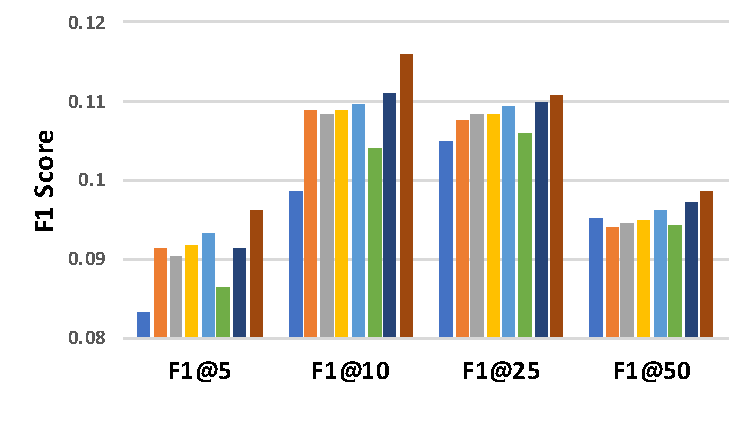
\includegraphics[width=\linewidth]{fig/F1-score_music}
  \caption{F1@K on \emph{Music} data.}
  \label{fig:perf_cmp_F1_music}
\endminipage\hfill
\minipage{0.32\textwidth}
  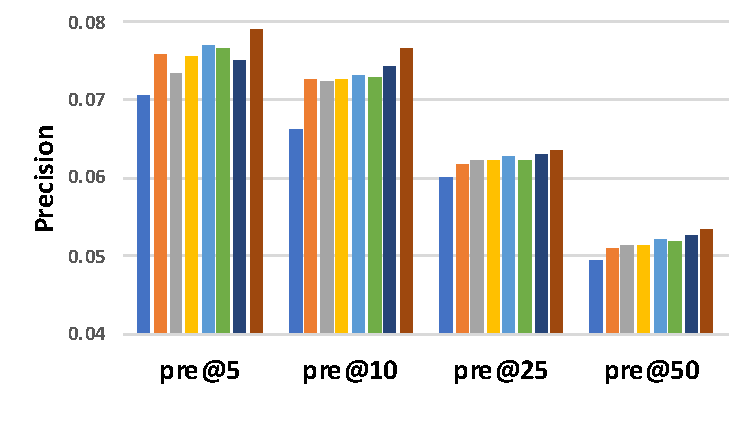
\includegraphics[width=\linewidth]{fig/precision_music}
  \caption{Precision@K on \emph{Music} data.}
  \label{fig:perf_cmp_precision_music}
\endminipage\hfill
\minipage{0.32\textwidth}%
  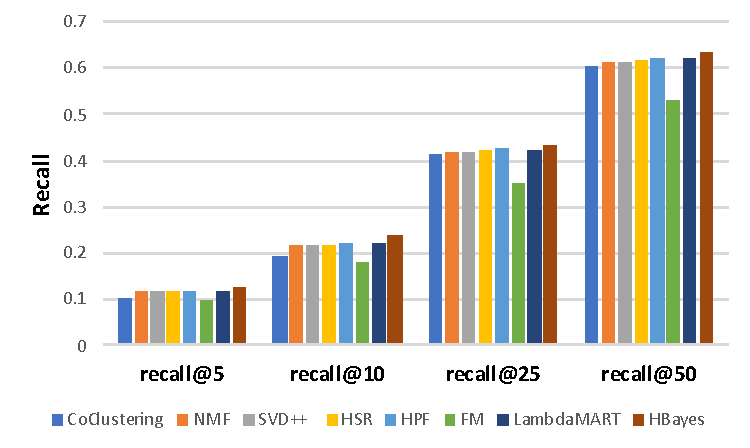
\includegraphics[width=\linewidth]{fig/recall_music}
  \caption{Recall@K on \emph{Music} data.}
  \label{fig:perf_cmp_recall_music}
\endminipage
\end{figure*}

\begin{figure}[!htb]
\centering
\minipage{0.49\columnwidth}
  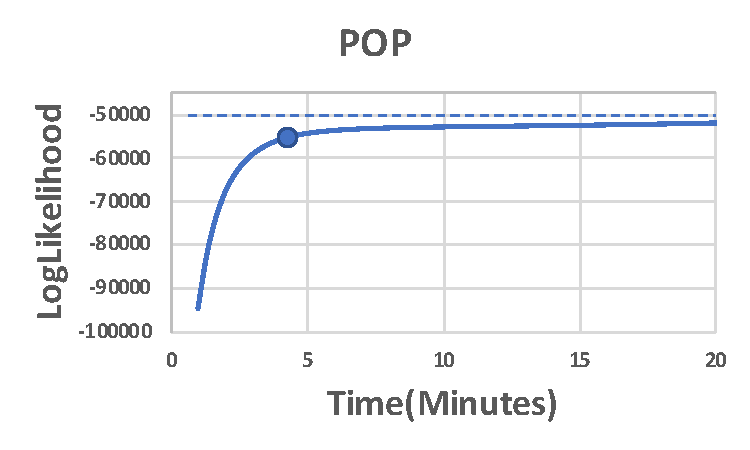
\includegraphics[width=\linewidth]{fig/1feature_lik}
\endminipage
\minipage{0.49\columnwidth}
  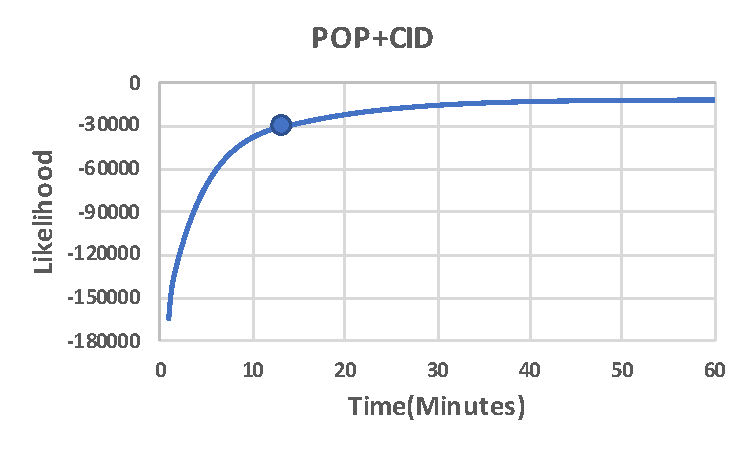
\includegraphics[width=\linewidth]{fig/2feature_lik}
\endminipage
\vskip\baselineskip
\minipage{0.49\columnwidth}
  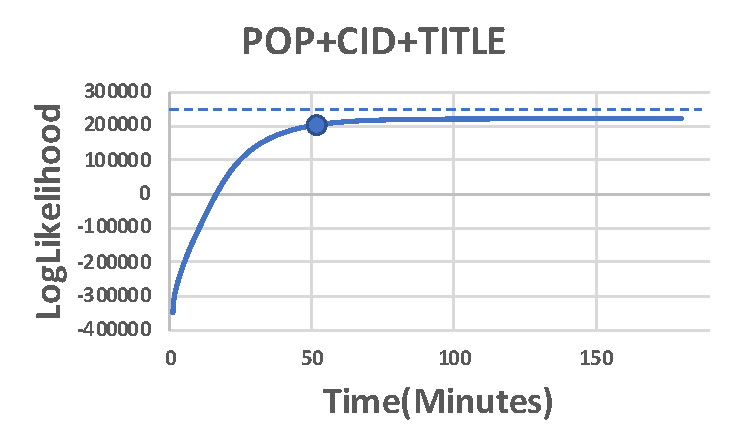
\includegraphics[width=\linewidth]{fig/3feature_lik}
\endminipage
\minipage{0.49\columnwidth}
  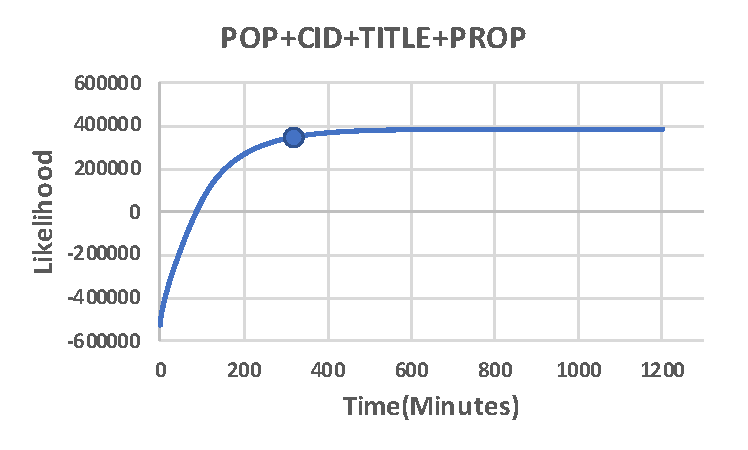
\includegraphics[width=\linewidth]{fig/4feature_lik}
\endminipage
\caption{Training time under different feature combinations on e-commerce recommendations}
\label{fig:train_time_cmp}
\end{figure}

%\begin{figure}[htb]
%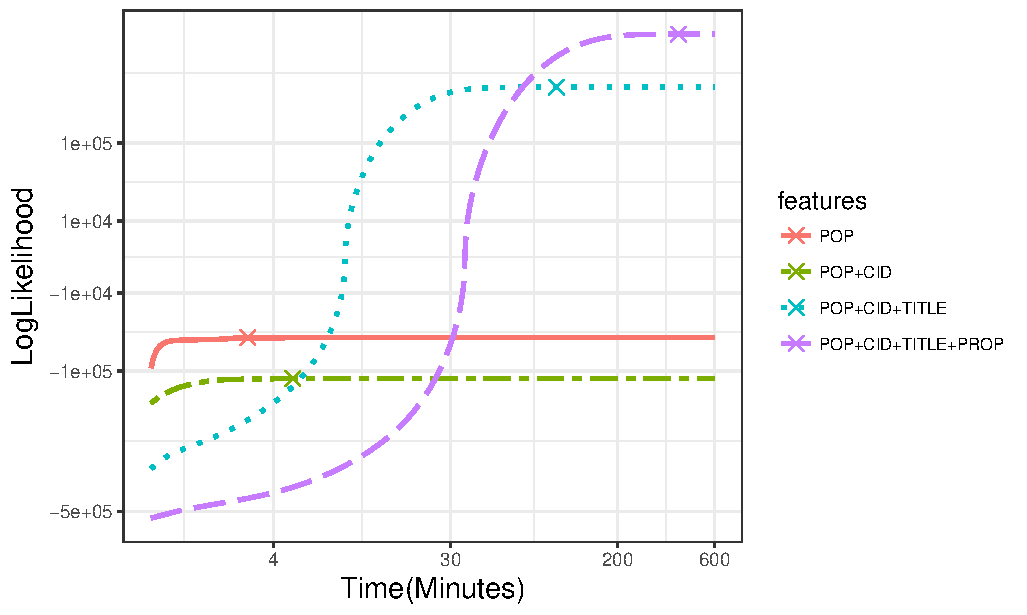
\includegraphics[width=0.9\columnwidth,height=0.5\columnwidth]{fig/Lik_time}
%\caption{Training time under different feature combinations on e-commerce recommendations}
%\label{fig:train_time_cmp}
%\end{figure}

\begin{table}[htb]
\begin{center}
\scalebox{0.85}{
\begin{tabular}{l|cccc}
\toprule
\textbf{Method} & \textbf{NDCG@5} & \textbf{NDCG@10} & \textbf{NDCG@25} & \textbf{NDCG@50} \\
\hline
\rowcolor{mygray}
CoClustering & 0.1288 & 0.1637 & 0.2365 & 0.3050 \\
NMF & 0.1249 & 0.0156 & 0.2272 & 0.3020 \\
\rowcolor{mygray}
SVD++ & 0.1138 & 0.1487 & 0.2287 & 0.3073\\
HSR & 0.1266 & 0.1603 & 0.2354 & 0.3107 \\
\rowcolor{mygray}
HPF & 0.1412 & 0.1757 & 0.2503 & 0.3229 \\
FM & 0.1363 & 0.1592 & 0.2291 & 0.3117\\
\rowcolor{mygray}
LambdaMART & 0.1287 & 0.1585 & 0.2304 & 0.3123\\
HBayes & \textbf{0.1557} & \textbf{0.1974} & \textbf{0.2871} & \textbf{0.3590}\\
\bottomrule
\end{tabular}}
\end{center}
\caption{NDCG on apparel recommendations}
\label{NDCG_cmp}
\end{table}

\subsubsection{Performance Comparison}
We first report the model performance regarding precision, recall, as well as F1-score for HBayes against other baselines in Figure (\ref{fig:perf_cmp_F1_apparel},\ref{fig:perf_cmp_precision_apparel},\ref{fig:perf_cmp_recall_apparel}).  As shown, when each method recommends fewer number of products (K = 5), HBayes does not show the superiority regarding with recalls, with the increment of recommended items, the recall for HBayes becomes much better against others, which implies HBayes is really efficient in terms of finding items that people tend to take interest in.  In the sense of precision, HBayes is consistently better than other baseline methods which implies HBayes is much more accurate in terms of item classification under different K.   Given the performance of precisions and recalls, HBayes is much better regarding F1-score with different K for apparel recommendation.

Regarding the ranking quality, we use NDCG to report each method's performance in Table (\ref{NDCG_cmp}).  HBayes is superior against other baseline methods through out different K recommended.  Specially, HBayes beats the second best HPF at $\text{K}=5$ by $10.3\%$, at $\text{K}=10$ by $12.4\%$, at $\text{K}=25$ by $14.7\%$ and at $\text{K}=50$ by $11.2\%$.  

\subsubsection{Model Learning Analysis}
\begin{figure}
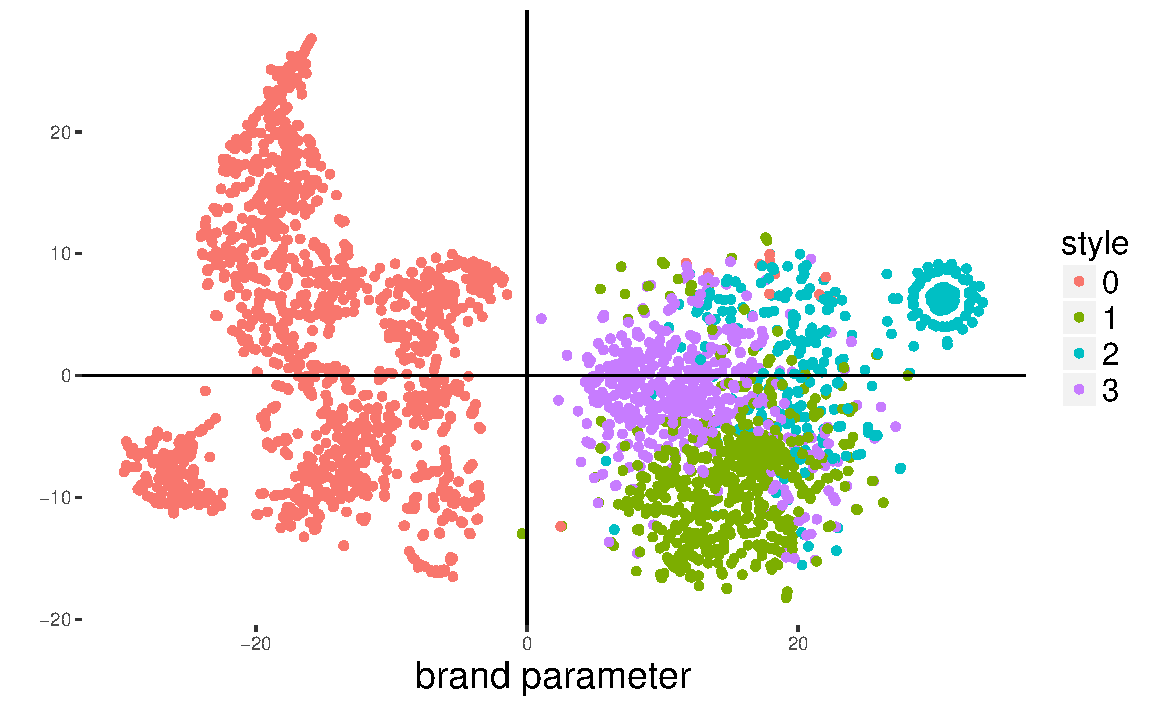
\includegraphics[width=0.58\columnwidth,height=3cm]{fig/brand_tsne}
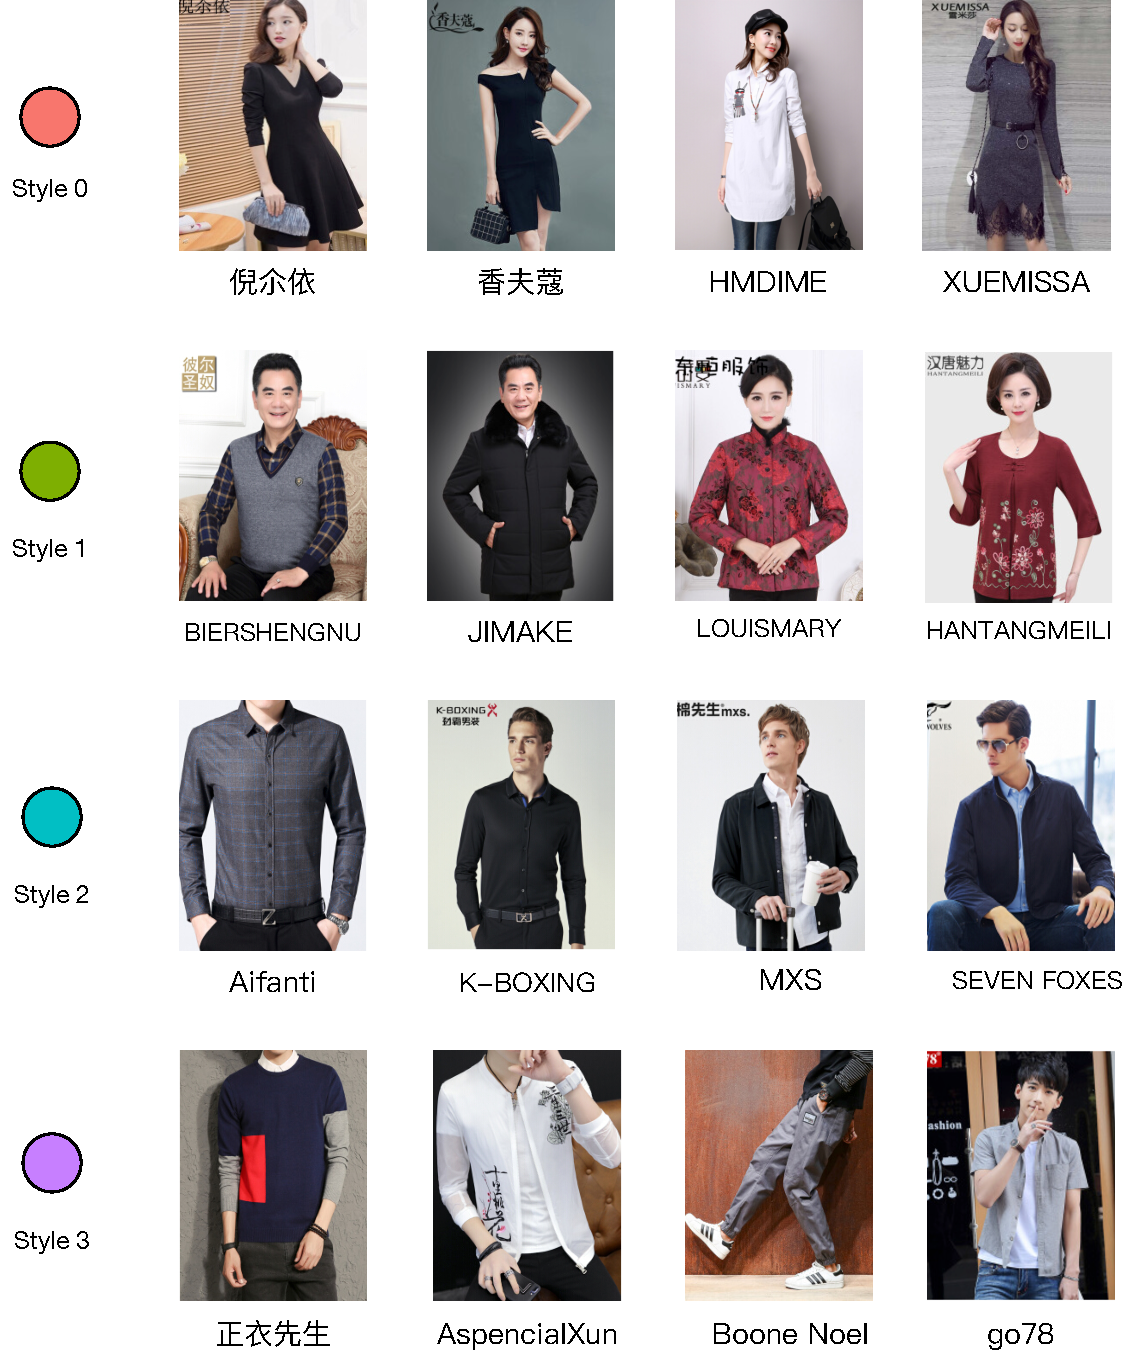
\includegraphics[width=0.39\columnwidth,height=4cm]{fig/style-brand}
\caption{tSNE of four latent apparel style clusters}
\label{fig:tsne-represntation-style-cluster}
\end{figure}

Like mentioned in Sec.\ref{sec:method}, HBayes learns the latent style clusters, and group different brands of products based on their different hidden style representations.  Figure (\ref{fig:tsne-represntation-style-cluster}) shows the tSNE \cite{maaten2008visualizing} representations of different apparel clusters learned by HBayes and we randomly pick $4$ samples out of each cluster and display each product image at the right subfigure.  As shown, cluster one which takes the majority proportion of apparel items seems about stylish female youth garment.  This intuitively makes sense because the majority of apparel customers are female youth for e-commerce websites; as a result, most apparels are focusing on the young female audience as well.    The second cluster seems about senior customers who are elder in age.   Interestingly, the third cluster and the fourth cluster that are closely tied up are both about male customer youth.  However, the third cluster seems focusing more on office business garment while the fourth cluster seems more about Korean-pop street styles.  This indicates us that the HBayes indeed learns the meaningful intrinsic garment styles from apparel items by leveraging customer behavior data.   

\subsection{Recommendation on Last.fm Music Data}
The second data set is collected from Last.fm dataset \cite{Celma:Springer2010} and Free Music Archive (FMA) \cite{FMA}. Last.fm is a publicly available dataset which contains the whole listening habits (till May, 5th 2009) for $\mathbf{1000}$ users. FMA is an open and easily accessible dataset providing $\mathbf{917}$ GiB and $\mathbf{343}$ days of Creative Commons-licensed audio from $\mathbf{106574}$ tracks, $\mathbf{16341}$ artists and $\mathbf{14854}$ albums, arranged in a hierarchical taxonomy of $\mathbf{161}$ genres. It also provides full-length and high-quality audios with precomputed features.  In our experiment, tracks in Last.fm dataset were further intersected with FMA dataset for better feature generation.  The resulting dataset contains $\mathbf{500}$ users, $\mathbf{16328}$ tracks and $\mathbf{36}$ genres.

\subsubsection{Performance Comparison}
We conduct similar experiments as we do for apparel dataset and report precisions, recalls as well as F1-scores in Figure (\ref{fig:perf_cmp_F1_music},\ref{fig:perf_cmp_precision_music},\ref{fig:perf_cmp_recall_music}).  Although HPF and HBayes share similar performance regarding recalls along with different K, HBayes is dominant for precisions at different K, especially when K is small (5, 10), which indicates HBayes is very efficient and precise for helping users pick up the songs they prefer even when the recommended item lists are short.   Combining the two, HBayes is superior in terms of F1-scores for different K recommended.  

For ranking qualities, we report the NDCG performance in Table (\ref{NDCG_cmp_music}).  Similar as e-commerce apparel data, HBayes is the best approach and HPF is the second best one throughout different K items recommended.  Specifically, HBayes beats HPF for $2.7\%$ at $\text{K}=5$, $4.3\%$ at $\text{K}=10$, $2.1\%$ at $\text{K}=25$, and $2.5\%$ at $\text{K}=50$ separately.

\begin{table}[htb]
\begin{center}
\scalebox{0.85}{
\begin{tabular}{l|cccc}
\toprule
\textbf{Method} & \textbf{NDCG@5} & \textbf{NDCG@10} & \textbf{NDCG@25} & \textbf{NDCG@50} \\
\hline
\rowcolor{mygray}
CoClustering & 0.2415 & 0.2314 & 0.2289 & 0.2349 \\
NMF & 0.2556 & 0.2494 & 0.2368 & 0.2431 \\
\rowcolor{mygray}
SVD++ & 0.2493 & 0.2478 & 0.2381 & 0.2439\\
HSR & 0.2544 & 0.2495 & 0.2384 & 0.2448\\
\rowcolor{mygray}
HPF & 0.2584 & 0.2513 & 0.2405 & 0.2474\\
FM & 0.2527 & 0.2453 & 0.2284 & 0.2333\\
\rowcolor{mygray}
LambdaMART & 0.2372 & 0.2337 & 0.2272 & 0.2218\\
HBayes & \textbf{0.2655} & \textbf{0.2620} & \textbf{0.2455} & \textbf{0.2537}\\
\bottomrule
\end{tabular}}
\caption{NDCG on Last.fm recommendations}
\label{NDCG_cmp_music}
\end{center}
\end{table}

%For PR-AUC, HBayes (0.055) again beats against the second best, which is LambdaMART (0.043) by $27.9\%$.  In terms of F1-score, HBayes in average beats against LambdaMART by $14.0\%$.  Regarding with the ranking quality, HBayes beats against the second best, which is NMF  for $M=5,10,25$ by $4.20\%$ in average and SVD++ for $M=50$ by $4.02\%$.  











\section{Conclusion(Chris)}
\label{sec:conclusion}


%\begin{figure}[h]
%\vspace{1in}
%\caption{Sample Figure Caption}
%\end{figure}

%\subsubsection*{References}

\bibliography{UAI2018}
\bibliographystyle{icml2018} % temporarily

\end{document}
